\section{The lifecycle of AI Models}

\as{What I miss here, and in fact I already missed it in the previous section, is a sort of roadmap: why are we talking about life-cycle now? Why did we enumerate types of models in the previous section? In what way are all these pieces connected, and how are they useful (or even necessary) for building "foundations for human-centered AI"?  I guess we should give such a roadmap in the Introduction, or even in a section by itself after the Introduction.}

In this section we describe the main phases of an AI model. These
phases can be the result of human intervention, automatic 
procedure, or a combination of the two.
\todo{Put the model lifecycle in a standard notation, e.g.,
  UML or BPMN, Emphasize the human interaction in the life cycle and the
interaction with the AI models \ps{I attempted both, see figure~\ref{fig:peterlifecycle}}}

\begin{figure}
\begin{center}
\begin{tikzpicture}[thick,action/.style={shape=rectangle, rounded corners,
                     draw, anchor=center,
                     text width=10em, align=center,
                     top color=white, bottom color=blue!20,
                     inner sep=1ex},
                   model/.style={shape=circle,
                     draw, anchor=center,
                     text width=5em, align=center,
                     top color=white, bottom color=red!20,
                     inner sep=1ex},
            input/.style={shape=rectangle,
                     draw, anchor=center,
                     text width=8em, align=center,
                     top color=white, bottom color=green!20,
                     inner sep=1ex},
            output/.style={shape=rectangle,
                     draw, anchor=center,
                     text width=8em, align=center,
                     top color=white, bottom color=yellow!20,
                     inner sep=1ex}]
 \node[action] (spec) {Model schema specification};
 \node[model,below = of spec] (mschema) {Model schema};
 \node[action,below = of mschema] (inst) {Model instantiation};
 \node[model,below = of inst] (model) {instantiated model};
 \node[action,below = of model] (inference) {Inference with the model};
 \node[action,right = of inst] (revision) {Quality Control \& Maintenance, e.g., \textbf{Verification}};
 \node[input,left = of inst] (knowledge) {Knowledge about the
   environment, training data, constraints, \textbf{requirements}};
 \node[input,left = of inference] (request) {Service request + input
   data, \textbf{observations}};
 \node[input,right = of revision] (add_knowledge) {Additional
   knowledge, evaluation of performances, and satisfaction of the \textbf{requirements}}; 
 \node[output,right = of inference] (answer) {Answer, decision,
   preference, \textbf{explanations}, \dots};
 \node[circle,draw] at ($ (answer) !.5! (revision) $) (plus)
 {\large\bf +};
 \draw[->] (spec) -- (mschema);
 \draw[->] (mschema) -- (inst);
 \draw[->] (knowledge) -- (inst);
 \draw[->] (knowledge) -- (inst);
 \draw[->] (inst) -- (model);
 \draw[->] (model) -- (inference);
 \draw[->] (request) -- (inference);
 \draw[->] (inference) -- (answer);
 \draw[->] (model) -- (plus);
 \draw[->] (answer) -- (plus);
 \draw[->] (plus) -- (revision);
 \draw[->] (add_knowledge) -- (revision);
 \draw[->] (revision) -- (mschema);
 \draw[->] (revision) -- (model);
\end{tikzpicture}
\end{center}
\caption{\label{fig:ai-model-lifecylce} The lifecycle of an artificial
  intelligence model}
\end{figure}

\begin{figure}
    \centering
    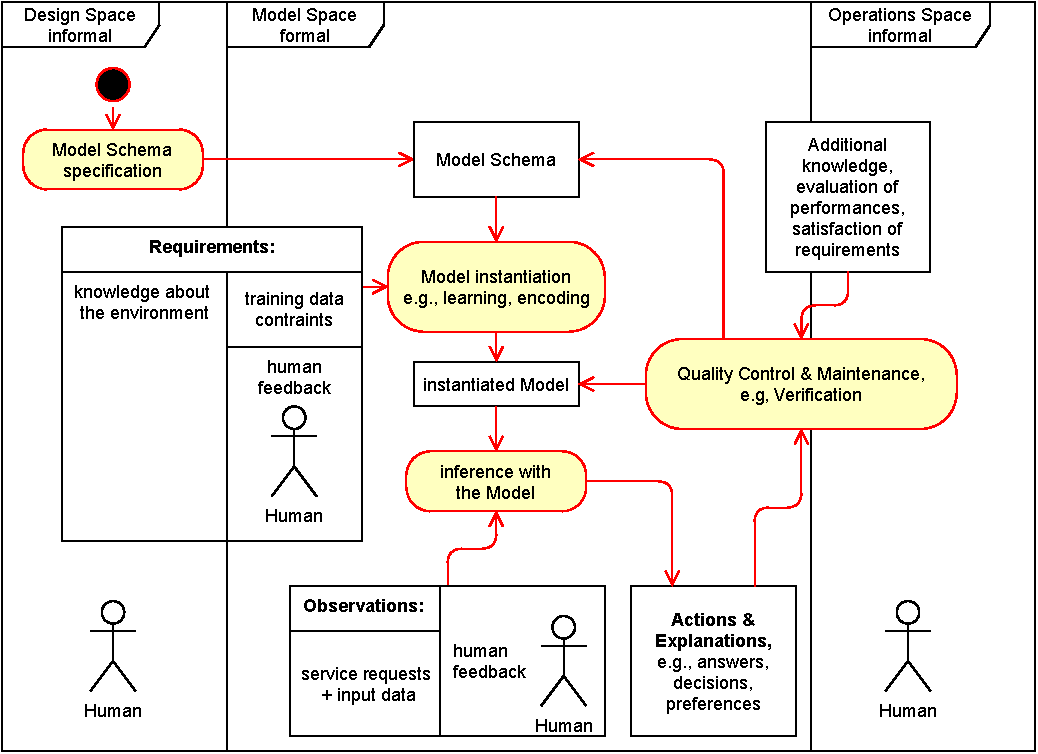
\includegraphics[width=\linewidth]{HCAI-lifecycle-v1}
    \caption{Lifecycle by Peter (v1)}
    \label{fig:peterlifecycle}
\end{figure}

\subsubsection{Model schema specification}

A model schema describes a class of models that shares the same structure. The models within the same class can be obtained by instantiating a (possibly infinite) set of parameters of the model schema (notice that here we use the term parameter in a very broad sense, referring both to the parameters of a probabilistic model, or a neural network, but also to the signature of logical language). Model schema specification is usually done manually, but there is a growing interest in the community in developing methods that (semi-)automatically learn the model structure from a set of observations/data. See for instance structural machine learning, programm sinthesis, non-parametric statistical models, auto-generated neural networks, predicate invention, and learning planning domains.

Associated to a model schema there is also an "intuitive explanation" of part of the models. For instance in choosing a logical lanague to specify the knowledge of an agent, one has to say for some fo the predicates what is the intuitive meaning (i.e., the meaning in the state of the environemt, i.e., the proposition) that is encoded by some predicate. Similarly in a neural network for classifying images in N classes C1,...,CN, one has to say which of the output neuron corresponds to each class Ci.

\subsubsection{Model instance specification/learning/update}

The instantiation of a model schema amounts in setting the "parameters" of the model. This amounts in encoding a certain amount of knowledge about the environment utilizing the "toolset" provided by the model schema. The encoding can be done manually, as often happens in logical rule based models via some knowledge engineering activity, or via supervised learning from data manually tagged by humans with labels, or in a complete unsupervised and automatic manner (e.g., clustering). Statistical models can be obtained by bayesian inference from a set of observations or by Maximum likelihood, or maximum a posteriori inference. Other methods for model specification can also be obtained by "model adaptation" and "transfer learning". Similarly update can be performed automatically via retraining, or manually, by modifying the parameters. Automatic learning of facts and rules from natural language is also possible. Methods for automatic learning of constraints from data are also available

\subsubsection{Inference with the model}
The second important aspect is how the model is used to infer a
decision i.e., an action that the artificial agent decides to
undertake. Given a set of observations $O$ as input, the model
provides as output a set of actions or a policy of actions. This is
obtained by applying an \emph{inference engine} which is defined on
the model.

In this phase the model instance is "queried" about what holds in the
environment. Inference can be very simple (like in neural network,
it's just the computation of the function) or rather complex as for
instance in constraint satisfaction in which it is necessary to apply
seart/optimizaiton algorithms. In logical model inference is done via
some form of logical reasoning (e.g., satisfiability) or model
checking, while in statistical model inference can be a generative
process (generate a data that has certain properties) or to compute
some marginal distribution of a certain (set of) stocastic
variables. What have in common all the above activities is that they
don't change the model they only query it.

\subsubsection{Quality Control and  Maintenance}
%edited by Peter
Once an AI artifact is ready to be used in practice,
additional tasks that are often not part of research activities become important
to reach higher Technology Readiness Levels.

%\begin{itemize}
%\item
For certification purposes and for the permission to use the artifact in practice on/with non-expert users, testing and verification procedures for safety/security-related properties of the behavior of the model can be necessary.
%
%\item
For products that are already in usage and needs to be updated,
maintenance and update methods need to exist so that problems that are identified after shipping the model can be counteracted.
%
%\item
For supporting users and for legal reasons, it can be necessary to have powerful methods for debugging model properties and (re-)actions and for explaining why certain outputs were (or were not) generated. Moreover, in connection with updates of the model, these methods can be useful to prove to authorities that certain behavior is excluded in the future.
%\end{itemize}

This part of the AI artifact lifecycle is very relevant to human-centric artificial intelligence, because it is the longest-lasting process in the existence of the model where the model has contact with a large number of untrained human individuals and unseen input data.


In the following we propose a high level summary of the different
techniques for schema model selection, model specification, learning
and update and inference in the model
